\documentclass[10pt,aspectratio=169]{beamer}
\tracinglostchars=0

\usetheme{Madrid}
\usecolortheme{default}

\usepackage{amsmath}
\usepackage{booktabs}
\usepackage{tikz}
\usepackage{xcolor}
\usetikzlibrary{arrows.meta,positioning,fit}

\definecolor{attnblue}{RGB}{0,102,204}
\definecolor{hotpink}{RGB}{255,38,142}
\definecolor{acid}{RGB}{255,220,0}
\definecolor{mint}{RGB}{37,190,140}
\definecolor{darkbg}{RGB}{29,36,45}
\definecolor{lightbg}{RGB}{245,245,250}

\setbeamercolor{structure}{fg=attnblue}
\setbeamercolor{frametitle}{bg=darkbg,fg=white}
\setbeamercolor{title}{bg=darkbg,fg=white}
\setbeamercolor{block title}{bg=attnblue!85!black,fg=white}
\setbeamercolor{block body}{bg=lightbg}
\setbeamercolor{alerted text}{fg=hotpink}
\setbeamercolor{author in head/foot}{bg=darkbg,fg=white}
\setbeamercolor{title in head/foot}{bg=attnblue!85!black,fg=white}
\setbeamercolor{date in head/foot}{bg=darkbg,fg=white}
\setbeamertemplate{navigation symbols}{}
\setbeamertemplate{footline}{%
  \leavevmode%
  \hbox{%
    \begin{beamercolorbox}[wd=.33\paperwidth,ht=2.25ex,dp=1ex,center]{author in head/foot}
      \normalfont\scriptsize syncopate-machine
    \end{beamercolorbox}%
    \begin{beamercolorbox}[wd=.34\paperwidth,ht=2.25ex,dp=1ex,center]{title in head/foot}
      \normalfont\scriptsize action IDs, not tokenizer text
    \end{beamercolorbox}%
    \begin{beamercolorbox}[wd=.33\paperwidth,ht=2.25ex,dp=1ex,right]{date in head/foot}
      \normalfont\scriptsize \insertframenumber{} / \inserttotalframenumber\hspace*{2ex}
    \end{beamercolorbox}}%
  \vskip0pt%
}

\title[Syncopate-Machine]{Syncopate-Machine}
\subtitle{Tiny Browser Transformer for Action-Sequence Chat}
\author{Dancing With My Code}
\date{Action-only architecture, 2026-05-25}

\begin{document}

\begin{frame}[plain]
  \titlepage
\end{frame}

\section{Contract}

\begin{frame}{The New Contract}
  \begin{center}
  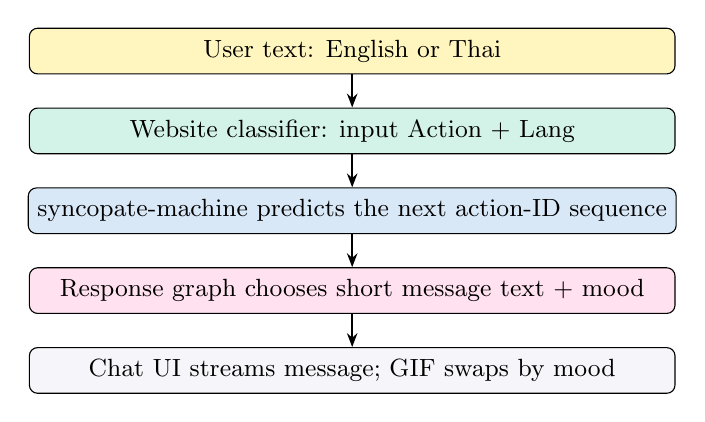
\begin{tikzpicture}[
    node distance=0.42cm,
    box/.style={draw,rounded corners=3pt,minimum width=8.2cm,
      minimum height=0.58cm,align=center,font=\small},
    arr/.style={-{Stealth[length=5pt]},thick}
  ]
    \node[box,fill=acid!25] (user) {User text: English or Thai};
    \node[box,fill=mint!20,below=of user] (classify)
      {Website classifier: input Action + Lang};
    \node[box,fill=attnblue!15,below=of classify] (model)
      {syncopate-machine predicts the next action-ID sequence};
    \node[box,fill=hotpink!14,below=of model] (graph)
      {Response graph chooses short message text + mood};
    \node[box,fill=lightbg,below=of graph] (ui)
      {Chat UI streams message; GIF swaps by mood};

    \draw[arr] (user) -- (classify);
    \draw[arr] (classify) -- (model);
    \draw[arr] (model) -- (graph);
    \draw[arr] (graph) -- (ui);
  \end{tikzpicture}
  \end{center}

  \smallskip
  \begin{block}{Hard rule}
    \small
    The model no longer predicts tokenizer pieces or raw words. It predicts
    \alert{action IDs}. Text is owned by the website response graph.
  \end{block}
\end{frame}

\begin{frame}{Why The Tokenizer Got Fired}
  \begin{columns}[T]
    \begin{column}{0.48\textwidth}
      \begin{block}{Old Path}
        \begin{itemize}
          \item SentencePiece tokenizer
          \item Text-token prediction
          \item Browser had to decode words
          \item More room for weird repeats
          \item Bigger checkpoint and slower UI
        \end{itemize}
      \end{block}
    \end{column}
    \begin{column}{0.48\textwidth}
      \begin{block}{New Path}
        \begin{itemize}
          \item No tokenizer at runtime
          \item 23 integer action IDs
          \item Website owns language and message style
          \item Mood is explicit for animation
          \item Tiny checkpoint, browser-friendly
        \end{itemize}
      \end{block}
    \end{column}
  \end{columns}

  \bigskip
  \centering
  \alert{Less magic. More control. Fewer stupid browser failures.}
\end{frame}

\section{Vocabulary}

\begin{frame}{Action Vocabulary}
  \small
  \centering
  \begin{tabular}{rll@{\hspace{0.9cm}}rll}
    \toprule
    \textbf{ID} & \textbf{Name} & \textbf{Role}
      & \textbf{ID} & \textbf{Name} & \textbf{Role} \\
    \midrule
     0 & PAD & padding       & 12 & Compliment & nice input \\
     1 & SOS & start         & 13 & Agree & yes / same \\
     2 & EOS & end           & 14 & Disagree & no / wrong \\
     3 & SEP & separator     & 15 & General & fallback \\
     4 & Unknown & unused fallback & 16 & Eating & food talk \\
     5 & Greeting & hello    & 17 & DailyLife & casual life \\
     6 & Farewell & goodbye  & 18 & RustGo & Rust beats Go \\
     7 & Frustrated & annoyed & 19 & Identity & who am I \\
     8 & Sad & low mood      & 20 & ShitTalk & roast mode \\
     9 & Happy & upbeat      & 21 & TH & Thai \\
    10 & Question & question  & 22 & EN & English \\
    11 & Insult & user swears &    &    & \\
    \bottomrule
  \end{tabular}
\end{frame}

\section{Model}

\begin{frame}{Tiny Model Shape}
  \begin{columns}[T]
    \begin{column}{0.45\textwidth}
      \begin{block}{Browser Model}
        \begin{tabular}{lr}
          \toprule
          Vocab & 23 \\
          Context & 64 \\
          Layers & 1 \\
          Width & 64 \\
          Attention heads & 4 \\
          KV heads & 1 \\
          FFN width & 64 \\
          Params & 24,192 \\
          \bottomrule
        \end{tabular}
      \end{block}
    \end{column}
    \begin{column}{0.5\textwidth}
      \begin{block}{Decoder Block}
        \begin{itemize}
          \item RMSNorm
          \item Causal attention (\alert{HigherOrder} polynomial kernel)
          \item RoPE position rotation
          \item Grouped-query attention
          \item SwiGLU feed-forward
          \item Weight-tied output projection
        \end{itemize}
      \end{block}
    \end{column}
  \end{columns}

  \bigskip
  \centering
  The neural model decides \alert{what kind of reply happens next};
  the website decides \alert{what words hit the chat box}.
\end{frame}

\begin{frame}{Parameter Count}
  \small
  Config: $V=23$, $N=1$, $d=64$, $n_h=4$, $n_{kv}=1$, $d_k=16$,
  $d_{ff}=64$

  \medskip
  \centering
  \begin{tabular}{llr}
    \toprule
    \textbf{Component} & \textbf{Formula} & \textbf{Params} \\
    \midrule
    Embedding & $V \times d = 23 \times 64$ & 1,472 \\
    Attention per layer & $d^2 + 2dn_{kv}d_k + d^2$ & 10,240 \\
    FFN per layer (SwiGLU) & $3dd_{ff}$ & 12,288 \\
    Norms per layer & $2d$ & 128 \\
    Final norm & $d$ & 64 \\
    \midrule
    Total & $1472 + 1(10240 + 12288 + 128) + 64$ & \alert{24,192} \\
    \bottomrule
  \end{tabular}

  \medskip
  Output projection reuses the embedding matrix, so it adds zero new params.
\end{frame}

\begin{frame}{Attention Kernels}
  \begin{columns}[T]
    \begin{column}{0.48\textwidth}
      \begin{block}{Softmax (default)}
        \[
          w = \texttt{softmax}\!\left(\frac{QK^\top}{\sqrt{d_k}} \cdot M\right)
        \]
        \begin{itemize}
          \item Standard scaled dot-product
          \item $\exp$ / $\sum$ normalization
          \item Well-studied, universally used
        \end{itemize}
      \end{block}
    \end{column}
    \begin{column}{0.48\textwidth}
      \begin{block}{\alert{HigherOrder} (active)}
        \[
          W = S \cdot K,\quad w = \frac{W W^\top \cdot K}{\sum|W W^\top|}
        \]
        \begin{itemize}
          \item Second-order polynomial kernel
          \item No $\exp$ — cheaper on weak GPUs
          \item \alert{Zero extra parameters}
        \end{itemize}
      \end{block}
    \end{column}
  \end{columns}

  \bigskip
  \centering
  $S$ = raw scores, $K$ = causal keep mask. Switch with \texttt{-{}-kernel} at train time.
\end{frame}

\section{Architecture Decision}

\begin{frame}{Why Not Bahdanau Attention?}
  \begin{columns}[T]
    \begin{column}{0.48\textwidth}
      \begin{block}{Bahdanau + GRU}
        \begin{itemize}
          \item Single-head additive attention
          \item Sequential decoding (step by step)
          \item GRU gates: $3 \times$ (input + hidden + bias)
          \item 1 GRU layer $\approx$ 2 transformer layers
          \item 1-layer $\approx$ 72K, 2-layer bi $\approx$ 291K params
          \item Training 2–3$\times$ slower
        \end{itemize}
      \end{block}
    \end{column}
    \begin{column}{0.48\textwidth}
      \begin{block}{Transformer + GQA (chosen)}
        \begin{itemize}
          \item Multi-head attention
          \item Parallel over all positions
          \item GQA \texttt{kv\_heads=1} is a cheat code
          \item K,V projections: $64 \times 16 = 1{,}024$ each
          \item \alert{24K params} for the full model
          \item Training $\sim$41 steps/s
        \end{itemize}
      \end{block}
    \end{column}
  \end{columns}

  \bigskip
  \centering
  Bahdanau shines for large seq2seq (translation). \alert{For tiny action-ID tasks, the transformer wins.}
\end{frame}

\begin{frame}{71K $\to$ 24K ($-66\%$)}
  \centering
  \begin{tabular}{lrr}
    \toprule
    \textbf{Setting} & \textbf{Before} & \textbf{After} \\
    \midrule
    Layers & 2 & 1 \\
    FFN intermediate & 128 & 64 \\
    Total params & 71,192 & 24,192 \\
    Val accuracy & --- & 63.2\% \\
    Perplexity & --- & 3.03 \\
    Training speed & --- & $\sim$41 steps/s \\
    \bottomrule
  \end{tabular}

  \bigskip
  \begin{block}{What changed}
    Halved decoder layers from 2~$\to$~1 and FFN width from 128~$\to$~64.
    Removed dead code: \texttt{SyncopateParameterBudget} enum,
    legacy preset methods.
    Active attention kernel: \alert{HigherOrder} (polynomial normalization,
    zero extra params vs Softmax).
    4 tests remain, all passing.
  \end{block}
\end{frame}

\begin{frame}{Browser Runtime}
  \begin{itemize}
    \item Website loads \texttt{model-personal-v2.mpk}
    \item Website loads \texttt{model-config-personal-v2.json}
    \item Runtime tries WebGPU first when requested
    \item Auto mode falls back to CPU when WebGPU is unavailable
    \item Chrome without a valid WebGPU adapter should not kill the chat box
    \item UI streams message text from graph output, not raw model tokens
  \end{itemize}

  \bigskip
  \begin{block}{Mood Contract}
    Model output action sequence maps to one mood:
    \texttt{normal}, \texttt{happy}, \texttt{frustrated}, or \texttt{sad}.
    The mascot GIF changes from that mood.
  \end{block}
\end{frame}

\begin{frame}{Training Path}
  \begin{block}{Data Build}
    \texttt{python examples/build\_action\_data.py --offline}
  \end{block}

  \begin{block}{CUDA Training}
    \small
    \texttt{cargo run --release --features cuda --example train\_action\_model --}\\
    \texttt{\quad --steps 3000 --batch-size 32 --lr 0.003}\\
    \texttt{\quad --kernel higher-order}\\
    \texttt{\quad --checkpoint-dir runs/action-higher-order}
  \end{block}

  \begin{itemize}
    \item Training is CUDA-only by design.
    \item Website runtime can choose WebGPU or CPU.
    \item Training data is action sequences, not text-token corpora.
  \end{itemize}
\end{frame}

\section{Cleanup}

\begin{frame}{What Got Deleted}
  \begin{columns}[T]
    \begin{column}{0.48\textwidth}
      \begin{block}{Removed Code}
        \begin{itemize}
          \item \texttt{ChatModel}
          \item \texttt{Trainer}
          \item \texttt{infer\_tokens*}
          \item old token generation APIs
          \item legacy layout engine
          \item old Multiscreen modules
        \end{itemize}
      \end{block}
    \end{column}
    \begin{column}{0.48\textwidth}
      \begin{block}{Removed Junk}
        \begin{itemize}
          \item SentencePiece experiment folder
          \item \texttt{spm\_train.exe}
          \item dead tokenizer examples
          \item obsolete tests
          \item stray ignored \texttt{nul} file
        \end{itemize}
      \end{block}
    \end{column}
  \end{columns}

  \bigskip
  \centering
  Remaining crate surface: \alert{action model + training + browser runtime}.
\end{frame}

\begin{frame}{Deploy Shape}
  \begin{itemize}
    \item Build the Leptos site with \texttt{trunk build --release}
    \item Ship the generated \texttt{dist/} directory to Vercel
    \item Keep model assets in \texttt{dancing-with-my-code-v2/assets/}
    \item Cache \texttt{.mpk} and \texttt{.json} assets aggressively
    \item Do not ship old tokenizer artifacts
  \end{itemize}

  \bigskip
  \begin{block}{Final State}
    The website talks like Dancing With My Code. The model only nudges
    conversation flow by action IDs. Clean split, less nonsense.
  \end{block}
\end{frame}

\begin{frame}{References}
  \begin{itemize}
    \item Burn framework: \texttt{https://github.com/tracel-ai/burn}
    \item Bahdanau et al.\ (2014): Neural Machine Translation by Jointly Learning to Align and Translate
    \item RoPE / RoFormer: rotary position embeddings
    \item GQA: grouped-query attention
    \item SwiGLU: gated feed-forward block
    \item Project docs: \texttt{README.md} and \texttt{DEVLOG.md}
  \end{itemize}
\end{frame}

\end{document}
